\section{How much stereo geometry error is detectable?} \label{sec:visual}
While direct passthrough errors elicited a reaching response consistent with geometric predictions, the impact of IPD errors was significantly weaker than predicted. This suggests that the visual system may be robust to—or perhaps less sensitive to—IPD mismatches compared to rendering offsets. To determine if this reduced behavioral sensitivity corresponds to a higher perceptual detection threshold, we conducted a follow-up psychophysical experiment using a two-interval forced choice (2IFC) task.

% We found in Section~\ref{sec:exp1results} that the magnitude of misperception induced by IPD error is much smaller than predictions of the geometric model. This result shows the underlying mechanism for distance judgment is only weakly sensitive to stereo cues in the IPD error condition. We wondered if this would also make IPD error be less detectable than what stereo geometry predicts. The next set of experiments directly measured detection thresholds for IPD error and direct passthrough error using a two interval forced choice (2IFC) task. 

%In the strictest sense, the distance that someone blind reaches is not a direct measure of perceived distance. We have shown in the previous section it is subject to a level of baseline bias, when corrected, aligns with our geometric model for two of three error conditions but not IPD error. In this next set of experiments we directly measured the perceived visual distance of an object using a psychophysical paradigm to directly interrogate the effects of errors in stereo geometry on distance perception. We used a two-interval forced choice (2IFC) task to determine whether an object with a purposefully induced rendering or viewing error appeared closer or farther than the same object rendered and viewed with accurate stereo geometry -- a task that is only possible in a platform like the the one described in Section~\ref{sec:hmd_platform}. Each instance of this judgment was fast, which allowed us to accumulate enough trials to extract the detection threshold from the psychometric function. These error detection thresholds were used to test the efficacy of our geometric model.

%The underlying visuomotor mapping from vision to reaching is also a process that is plastic and adaptable \cite{krakauer2000learning}.

\subsection{Participants}
The same 32 participants that performed the reaching experiments participated in this study and all protocols were IRB approved.

\subsection{Methods}
In each trial, participants viewed a red sphere in two successive intervals: a reference interval (rendered with correct stereo geometry) and a comparison interval (rendered with either a direct passthrough or IPD error). The interval order was randomized, and each interval lasted 800 ms with a 200 ms inter-stimulus interval. Participants indicated which interval appeared closer via controller input. The monocular size of the sphere in the reference interval was always fixed at 1$^\circ$, but scaled naturally according to perspective geometry in the comparison interval. We used the Method of Constant Stimuli to sample the psychometric function, varying error magnitudes in 100 equal steps ($\pm 12$~mm for IPD; $\pm 100$~mm for direct passthrough). Each participant completed 1200 trials (2 error types $\times$ 3 distances $\times$ 2 scenes $\times$ 100 repetitions) in randomized order, separated into three blocks for each viewing distance.



\begin{figure}
	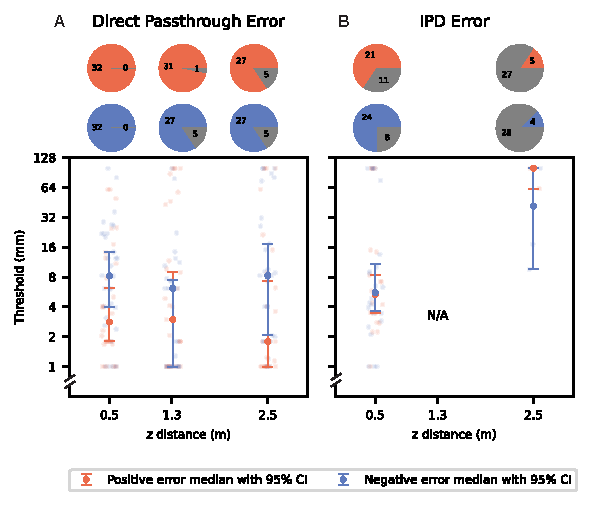
\includegraphics[width=\linewidth]{figures/visual/detection_thresholds_with_background.pdf}
	\caption{Detection thresholds for \textbf{(A)} direct passthrough error and \textbf{(B)} IPD error. Red and blue points are detection thresholds for positive and negative error directions. For IPD error, a positive error means HMD IAD is larger than user IPD and vice versa. For direct passthrough error, a positive error means rendering cameras are in front of HMD CoP and vice versa. Pie chart shows split of participants that were sensitive to the specific error type (red or blue) and sign vs those who performed at chance (gray). For target placed 1.3~m and affected by IPD error, our geometric model predicts no error and detection threshold is ill-defined.}
	\label{fig:detection_thresholds_with_background}
\end{figure}

\subsection{Viewing Conditions}
We expected sensitivity for both error types to depend on viewing distance and scene content. We varied distance and visual scene to explore the effects of three specific perceptual phenomenon.

% \begin{itemize}
    \paragraph{Stereo Sensitivity Gradient (IPD)} Binocular disparity cues degrade non-linearly with distance ($1/d^2$) \cite{howard2012perceiving}. We selected test distances of $0.5$~m (Near), $1.3$~m (Intermediate/VID), and $2.5$~m (Far). We hypothesized that IPD errors, which rely on disparity and vergence shifts, would be more detectable in the near field, undetectable at the VID (because viewing errors do not introduce geometric errors at the VID), and less detectable $2.5$~m.
    \paragraph{Weber's Law (Passthrough)} For direct passthrough, the rendering error represents a depth offset ($\Delta d$). According to Weber's Law, the Just Noticeable Difference (JND) should scale with total distance ($\Delta d / d = k$). Therefore, we expected thresholds to be lowest at $0.5$~m and highest at $2.5$~m.
    \paragraph{Cue Integration (Scene Content)} We utilized two environments to modulate cue reliability. A complex scene provided strong monocular cues (linear perspective, height-in-field) that may conflict with or override erroneous stereo cues. A sparse scene showed only a fixation target with a Skybox background, and this reduced scene may increase sensitivity to IPD errors compared to the structured environment.
% \end{itemize}

\subsection{Psychometric Function Fitting}
% \paragraph{Psychometric Function Fitting}
We excluded participants who were not sensitive enough to the combination of error type and error sign by performing a one-tailed binomial test (alpha value 0.05), which determines whether psychometric performance is different from chance (50\%). We estimated detection thresholds by fitting a psychometric function to the log-transformed error values for positive and negative errors separately. Additional details are provided in Supplementary Materials. 

% \paragraph{Linear Mixed Effect Modeling}
% Like the reaching experiments we specified another linear mixed effects model (LMEM) to evaluate the impact of error type, viewing distance, and background on each participant's detection threshold. The maximal model in for this analysis is:
% \begin{equation}
%     \text{threshold} \sim \text{distance} * \text{scene} + (\text{distance} * \text{scene} \mid \text{ID})
% \end{equation}
% where detection threshold was the best-fit threshold of a single participant's psychometric function. We used the beta coefficients and associated p-values for the fixed effect slope and intercept terms of interest to make statistical decisions.

\begin{figure}
	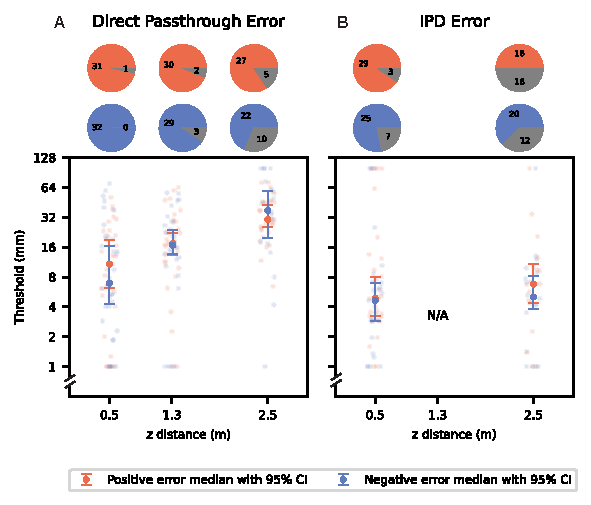
\includegraphics[width=\linewidth]{figures/visual/detection_thresholds_no_background.pdf}
	\caption{Detection thresholds for \textbf{(A)} direct passthrough error and \textbf{(B)} IPD error with only the skybox scene.
	}
	\label{fig:detection_thresholds_no_background}
\end{figure}


\subsection{Results} \label{sec:exp2results}
\paragraph{Error Detectability in Naturalistic Conditions}
We first assessed the absolute range of perceptible errors in the naturalistic environment (the Forest scene).  Overall we identify trends that are consistent with our expectations, IPD error is perceptible at near distances and nearly imperceptible at far distances (Figure~\ref{fig:detection_thresholds_with_background}B).  However, participants have a surprisingly high threshold for IPD errors, at approximately 6 mm. This relatively large error required for detection (approximately 10\%) is consistent with our reaching results, which show that IPD errors have a smaller than expected impact on reach distance. At intermediate ($1.3$~m) and far ($2.5$~m) distances, psychometric functions were predominantly flat, indicating that most participants could not distinguish the error from the reference. Additionally, at the VID, the geometric model predicts zero geometric distortion for viewing errors; consequently, an objective ground truth for "correct" interval identification—which is required to extract detection thresholds—is theoretically undefined.

To confirm whether participants were performing above chance, we applied a one-tailed binomial test to the psychometric fits. The results confirmed widespread insensitivity to IPD mismatches. Out of 64 fits at the far and intermediate distances, only 7 exhibited performance significantly above chance at the far distance resulting in an IPD detection threshold of $>$41 mm. Insensitivity persisted for some even at $0.5$~m, where stereo cues are strongest; 13 participants failed to exceed chance performance in at least the positive or negative IPD error conditions.

In contrast, participants were consistently sensitive to direct passthrough errors (Figure~\ref{fig:detection_thresholds_with_background}A). Median thresholds were between $1.8$--$3.0$~mm across viewing distances for positive errors, and $6.1$-$8.3$ for negative errors. Ulike IPD errors, the failure rate was minimal (only 16 failures total across all conditions), indicating a much more robust perceptual signal.

\paragraph{Scene Complexity}
In the naturalistic forest scene, depth cues other than stereopsis provide reliable distance information. In our sparse scene, where these other cues are removed, we observed that sensitivity to IPD errors improved dramatically, whereas sensitivity to direct passthrough errors decreased. Most notably, IPD viewing errors at the far distance were largely undetectable in the natural scene (55 of 64 psychometric functions), but detection rates improved significantly in the sparse scene (dropping to 28 of 64 undetectable cases). For participants who met the inclusion criteria in the sparse condition, median IPD error thresholds were 5.0 mm (negative) and 6.8 mm (positive) - a massive improvement from the 41.4 (negative) and 100 (negative) mm thresholds obtained from the 9 thresholds that met the inclusion criteria in the complex scene. At the near distance median IPD thresholds improved from 5.6 mm and 5.4 mm (natural) to 4.6 mm and 4.9 mm (sparse) for negative and positive errors, respectively. These results indicate that perceptual sensitivity to IPD errors is strongly dependent on scene content and increases when other depth cues are eliminated.

Conversely, sensitivity to direct passthrough rendering errors followed the opposite trend: median thresholds were substantially elevated (indicating lower sensitivity) across most conditions in the sparse scene. This is expected because the geometric impact of passthrough error diminishes as viewing distance increases. In the naturalistic scene, there are still objects located close to the viewer remain even when the target object is farther away, providing high-sensitivity references. The removal of these foreground objects in the sparse scene resulted in an approximately $3\times$ increase in thresholds at the far distance compared to the near distance.



% Participants' thresholds for direct passthrough error were higher overall in the skybox scene, and increased more rapidly as a function of viewing distance (1.13 mm vs. 0.355 mm per 1 m object distance; t = 3.06; p = 0.002 for the interaction of background presence and object distance). For IPD error, the opposite was observed (0.24 mm vs. 0.82 mm per 1 m object distance; t = -2.11; p = 0.036 on the same interaction). 
